\chapter{Objectives}
The project is based on the design, manufacture and characterization of an electrochemical biosensor on a flexible substrate to be used on the NanoPoc platform (Figure ~\ref{fig:Figura_Nano_Poc}), developed at the Instituto Nacional de Tecnología Industrial, for the detection of bacterial, viral or parasitic diseases in human and animal health \cite{PosterPoc2}.

\begin{figure}[H]
  \centering
    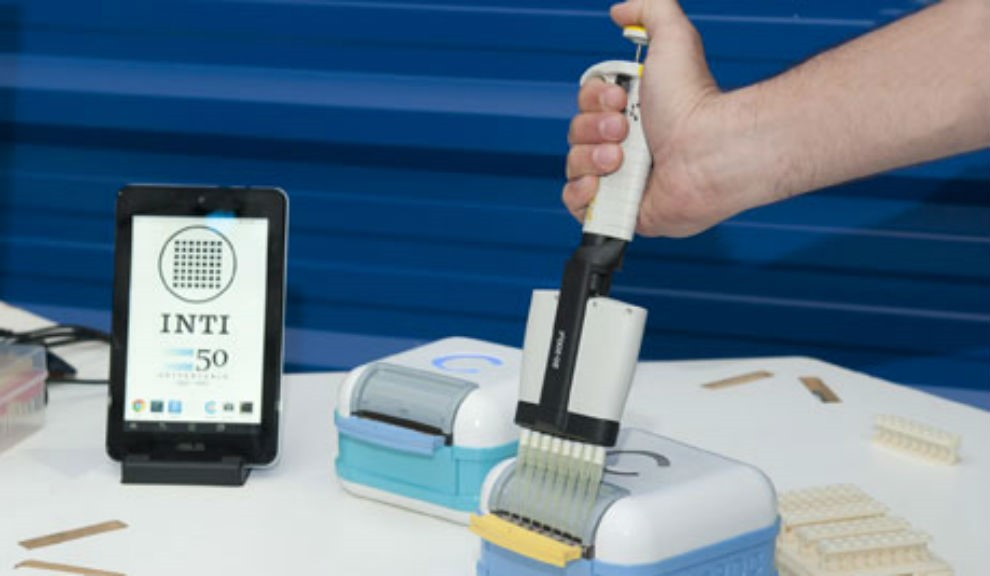
\includegraphics[width=0.5\textwidth]{Figures/Figura_Nano_Poc}
  \caption{NanoPoc platform.}
  \label{fig:Figura_Nano_Poc}
\end{figure}

\section{General Objectives}
The main objective is to generate a biosensor that is easy to manufacture and with high reproducibility. The aim is to improve its use, avoiding the handling of sample preparation between extraction and measurement in the device, for the $``$\textit{in situ}$"$ detection of infectious diseases in humans and animals, depending on the type of bioreceptor developed (Figure ~\ref{fig:Figura_Biosensor_objetivos}).

\begin{figure}[H]
  \centering
    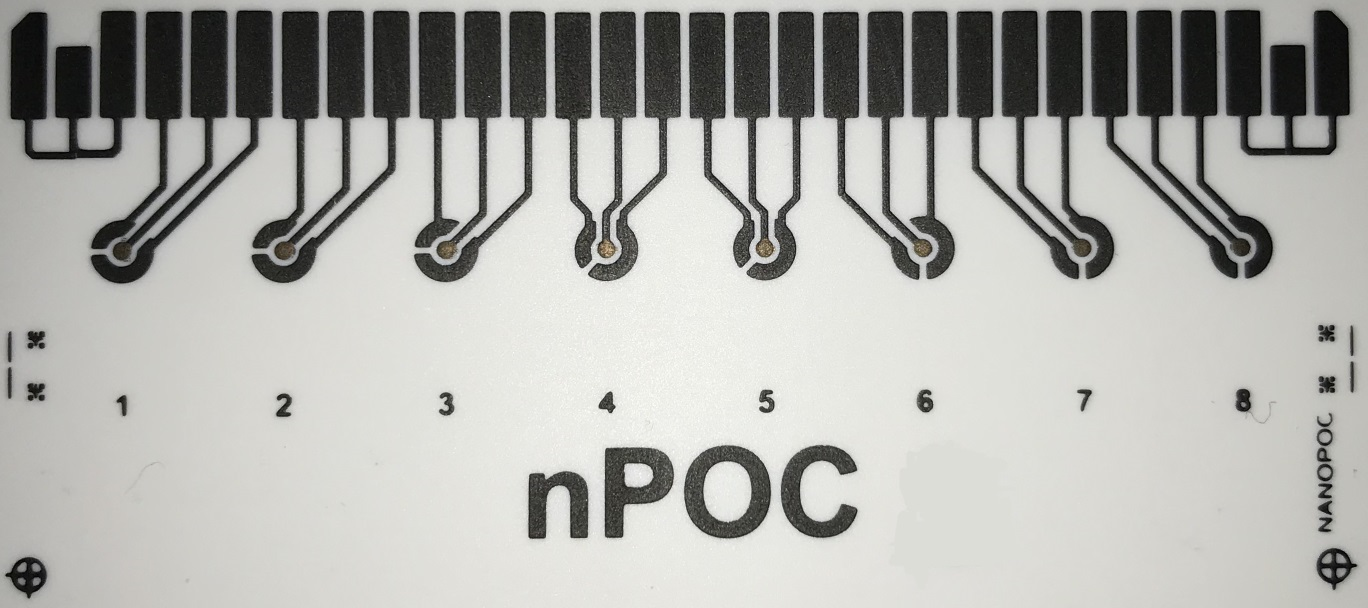
\includegraphics[width=0.5\textwidth]{Figures/Figura_Biosensor_objetivos}
  \caption{Biosensor.}
  \label{fig:Figura_Biosensor_objetivos}
\end{figure}

\section{Specific Objectives}
- Manufacture the sensors with the appropriate form, by means of a controlled deposition of material on the flexible substrate, creating 8 electrochemical cells with the standard dimensions of an 8-channel micropipette (Figure ~\ref{fig:Figura_celda_electroquimica}).\\

\begin{figure}[H]
  \centering
    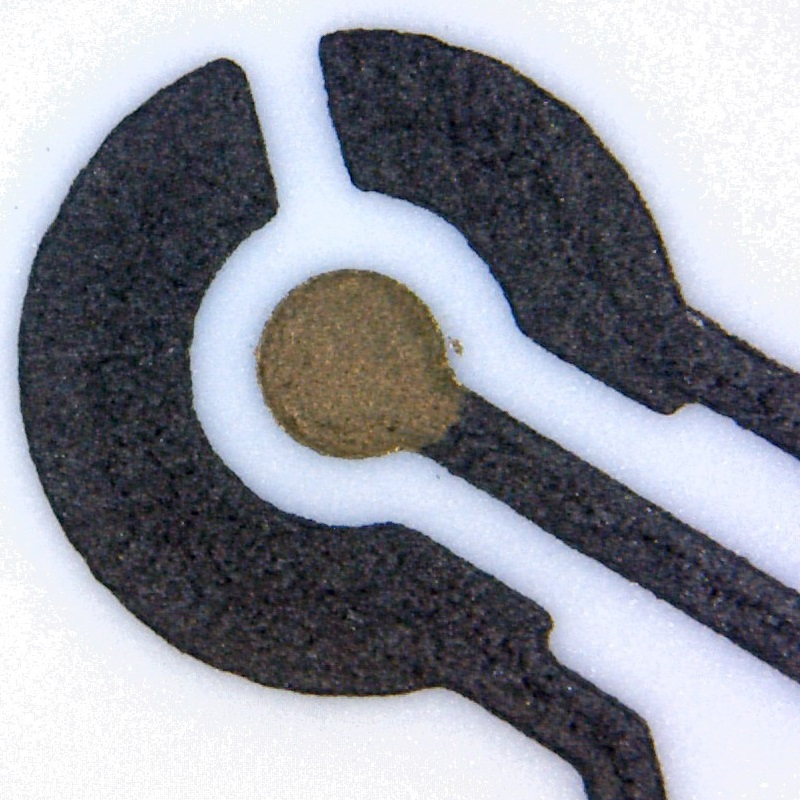
\includegraphics[width=0.35\textwidth]{Figures/Figura_celda_electroquimica}
  \caption{Electrochemical Cell.}
  \label{fig:Figura_celda_electroquimica}
\end{figure}

- Calibrate the inkjet printer in order to obtain the desired biosensor design using a specific ink on the chosen substrate (Figure ~\ref{fig:Figura_impresora_objetivos}).\\

\begin{figure}[H]
  \centering
    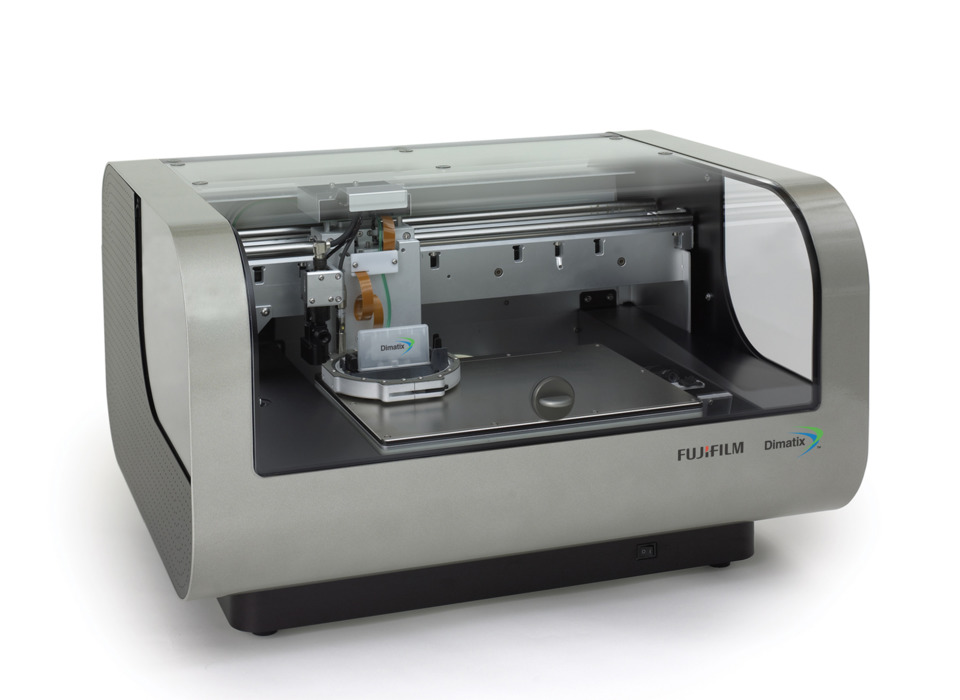
\includegraphics[width=0.5\textwidth]{Figures/Figura_impresora_objetivos}
  \caption{Inkjet Printer.}
  \label{fig:Figura_impresora_objetivos}
\end{figure}

- Obtain a correct response from the biosensors by means of a chemical solution equivalent to a specific analyte using the electrochemical technique of the amperometric type (Figure ~\ref{fig:Figura_caracElectroquim_objetivos}).\\

\begin{figure}[H]
  \centering
    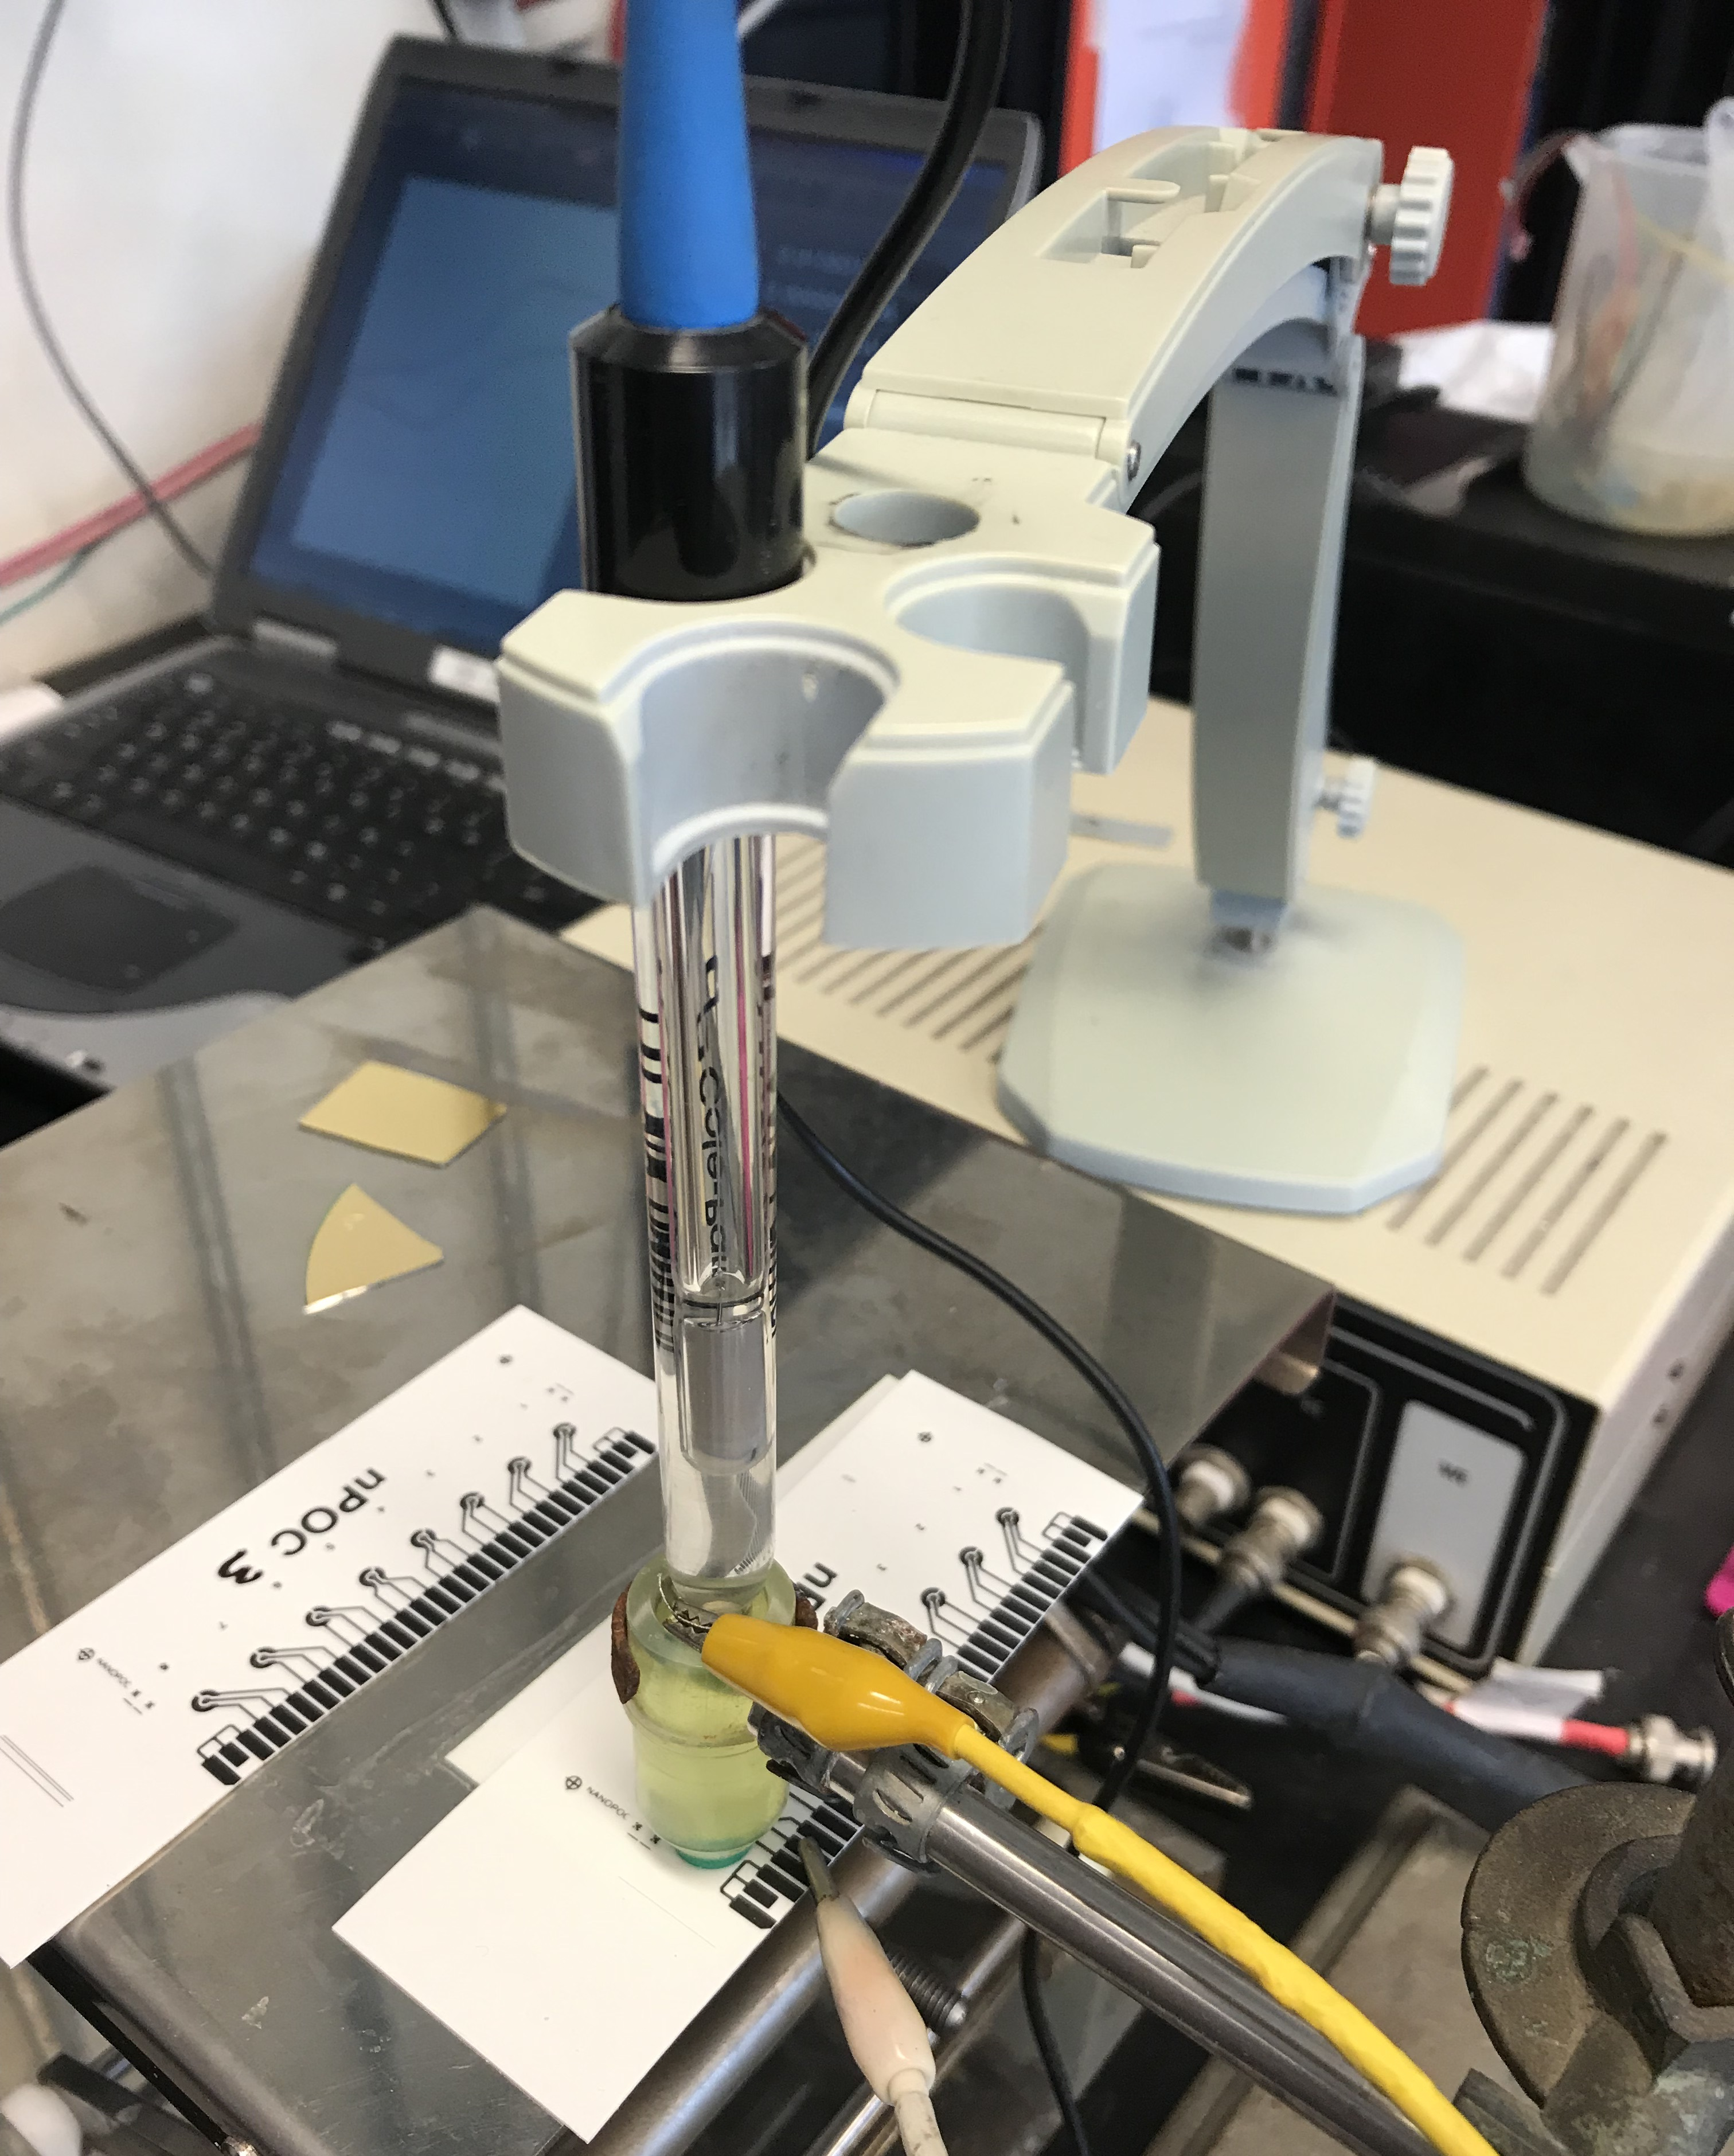
\includegraphics[width=0.4\textwidth]{Figures/Figura_caracElectroquim_objetivos}
  \caption{Electrochemical characterization.}
  \label{fig:Figura_caracElectroquim_objetivos}
\end{figure}